% Options for packages loaded elsewhere
\PassOptionsToPackage{unicode}{hyperref}
\PassOptionsToPackage{hyphens}{url}
%
\documentclass[
]{article}
\title{Reporte COVID}
\author{Luis Barrios}
\date{12/1/2022}

\usepackage{amsmath,amssymb}
\usepackage{lmodern}
\usepackage{iftex}
\ifPDFTeX
  \usepackage[T1]{fontenc}
  \usepackage[utf8]{inputenc}
  \usepackage{textcomp} % provide euro and other symbols
\else % if luatex or xetex
  \usepackage{unicode-math}
  \defaultfontfeatures{Scale=MatchLowercase}
  \defaultfontfeatures[\rmfamily]{Ligatures=TeX,Scale=1}
\fi
% Use upquote if available, for straight quotes in verbatim environments
\IfFileExists{upquote.sty}{\usepackage{upquote}}{}
\IfFileExists{microtype.sty}{% use microtype if available
  \usepackage[]{microtype}
  \UseMicrotypeSet[protrusion]{basicmath} % disable protrusion for tt fonts
}{}
\makeatletter
\@ifundefined{KOMAClassName}{% if non-KOMA class
  \IfFileExists{parskip.sty}{%
    \usepackage{parskip}
  }{% else
    \setlength{\parindent}{0pt}
    \setlength{\parskip}{6pt plus 2pt minus 1pt}}
}{% if KOMA class
  \KOMAoptions{parskip=half}}
\makeatother
\usepackage{xcolor}
\IfFileExists{xurl.sty}{\usepackage{xurl}}{} % add URL line breaks if available
\IfFileExists{bookmark.sty}{\usepackage{bookmark}}{\usepackage{hyperref}}
\hypersetup{
  pdftitle={Reporte COVID},
  pdfauthor={Luis Barrios},
  hidelinks,
  pdfcreator={LaTeX via pandoc}}
\urlstyle{same} % disable monospaced font for URLs
\usepackage[margin=1in]{geometry}
\usepackage{graphicx}
\makeatletter
\def\maxwidth{\ifdim\Gin@nat@width>\linewidth\linewidth\else\Gin@nat@width\fi}
\def\maxheight{\ifdim\Gin@nat@height>\textheight\textheight\else\Gin@nat@height\fi}
\makeatother
% Scale images if necessary, so that they will not overflow the page
% margins by default, and it is still possible to overwrite the defaults
% using explicit options in \includegraphics[width, height, ...]{}
\setkeys{Gin}{width=\maxwidth,height=\maxheight,keepaspectratio}
% Set default figure placement to htbp
\makeatletter
\def\fps@figure{htbp}
\makeatother
\setlength{\emergencystretch}{3em} % prevent overfull lines
\providecommand{\tightlist}{%
  \setlength{\itemsep}{0pt}\setlength{\parskip}{0pt}}
\setcounter{secnumdepth}{-\maxdimen} % remove section numbering
\ifLuaTeX
  \usepackage{selnolig}  % disable illegal ligatures
\fi

\begin{document}
\maketitle

\hypertarget{histuxf3rico-de-casos-covid-en-lima}{%
\subsection{Histórico de casos covid en
Lima}\label{histuxf3rico-de-casos-covid-en-lima}}

Como se puede observar estamos en la ``tercera ola'', aunque cabe
destacar que en esta ocasión el número de contagiados ha sobrepasado
largamente al pico de anteriores periodos. Esto debido a la nueva
variante OMICRON entre otros posibles factores.

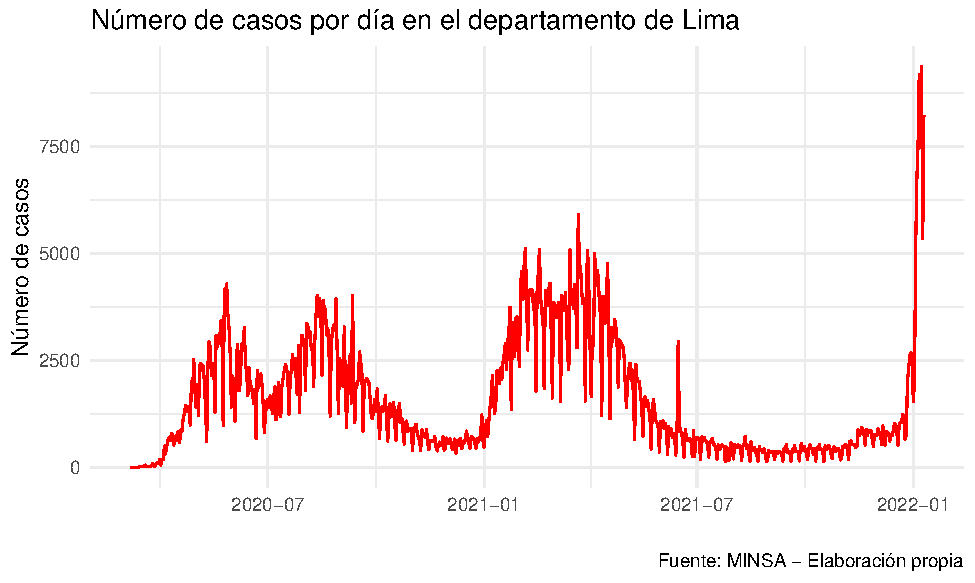
\includegraphics[width=0.8\linewidth]{reporte_covid_files/figure-latex/covid graphs-1}

\hypertarget{tendencia-reciente-de-casos-covid}{%
\subsection{Tendencia reciente de casos
covid}\label{tendencia-reciente-de-casos-covid}}

En el siguiente gráfico se puede observar la tendencia de los casos
confirmados durante las últimas tres semanas, como se puede observar,
aproximadamente desde el 26 de diciembre comienza a escalar el virus
nuevamente.

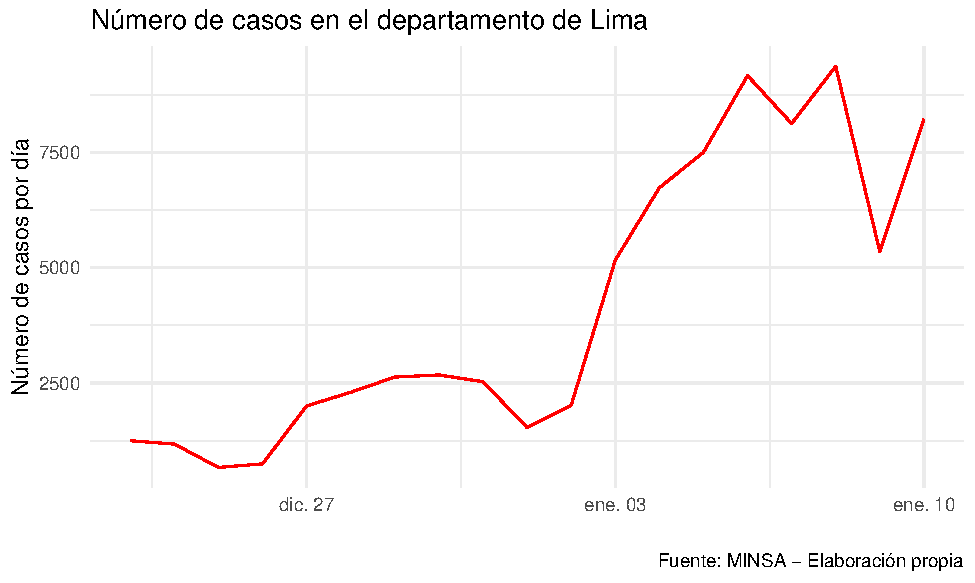
\includegraphics[width=0.8\linewidth]{reporte_covid_files/figure-latex/total -1}
\#\# Mapa Covid Enero 2022 El siguiente mapa representa el numero de
casos covid por departamento, un color más cercano al negro representa
un mayor número de contagiados, y viceversa, colores cercanos al blanco
significan contagios cercanos a cero, es notorio que la diferencia de
casos de contagiados entre Lima y los demás departamentos es abismal,
pero este puede ser un resultado sesgado dado que no se esta tomando en
cuenta que Lima tambien posee una cantidad de habitantes sumamente
superior a los demás.

\begin{verbatim}
## Reading layer `dp' from data source `C:\Users\LBarrios\Downloads\MAPA\dp.shp' using driver `ESRI Shapefile'
## Simple feature collection with 25 features and 13 fields
## Geometry type: MULTIPOLYGON
## Dimension:     XY
## Bounding box:  xmin: -81.32823 ymin: -18.35093 xmax: -68.65228 ymax: -0.03860597
## Geodetic CRS:  WGS 84
\end{verbatim}

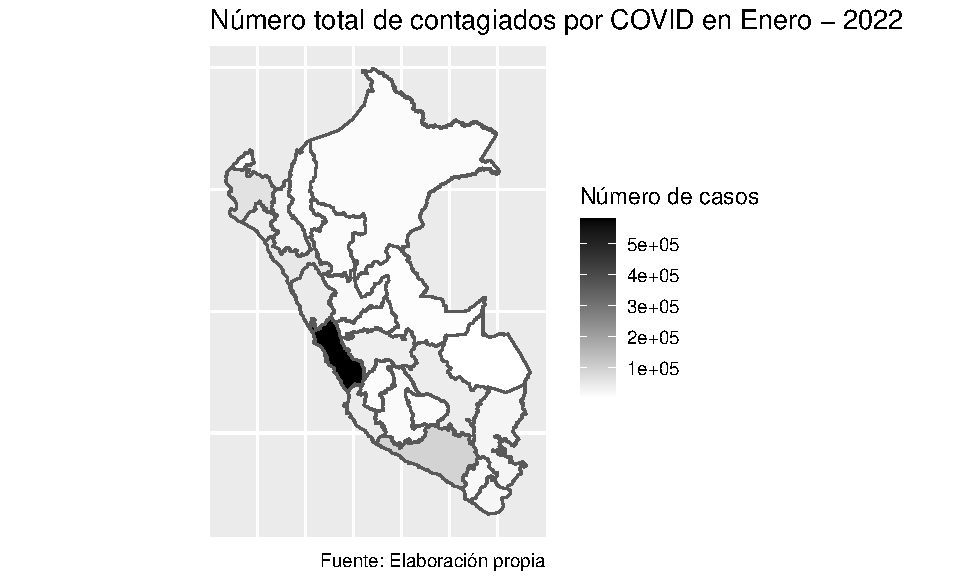
\includegraphics[width=0.8\linewidth]{reporte_covid_files/figure-latex/mapa1-1}
\#\# Mapa ratio Covid Por lo tanto se incluye la variable poblacion por
departamento en el análisis, siendo el ratio generado la división entre
el número de casos confirmados y el número de personas que habitan dicho
departamento, el ratio podría ser interpretado como el porcentaje de
personas que estan infectadas en determinado departamento, siendo por lo
tanto, un ratio mayor(color cercano a negro) un indicador de mayor
porcentaje de contagiados, en consecuencia, los departamentos más
cercanos al color negro estan en una pero situación sanitaria que
aquellos con colores cercanos al blanco.

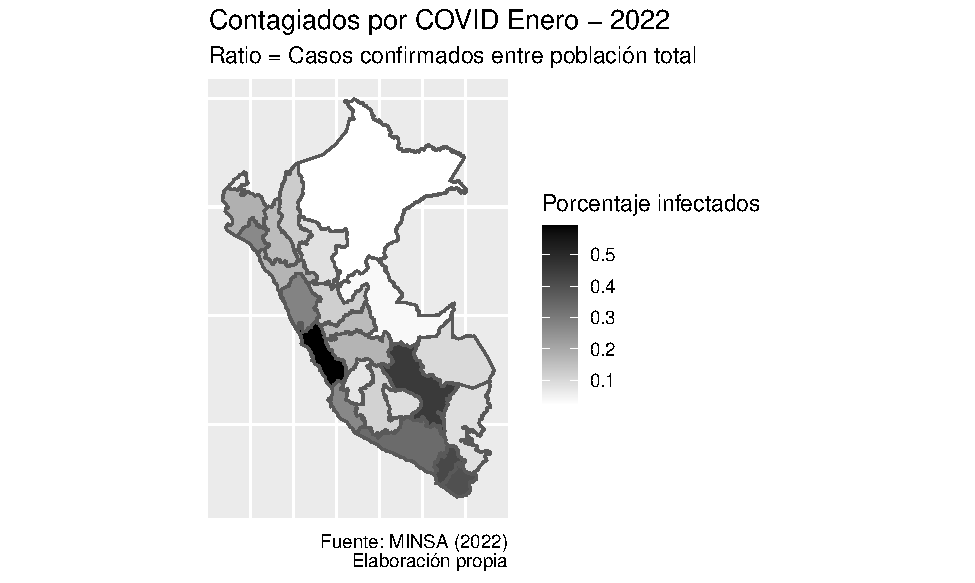
\includegraphics[width=0.8\linewidth]{reporte_covid_files/figure-latex/mapa2-1}

\end{document}
